\documentclass[11pt]{article}
\usepackage[margin=1in]{geometry}
\usepackage{amsmath,amssymb,mathtools}
\usepackage{booktabs,enumitem}
\usepackage{algorithm,algpseudocode}
\usepackage{microtype,needspace}
\usepackage{tikz}
\usetikzlibrary{arrows.meta,positioning}
\usepackage[hidelinks]{hyperref}
\newcommand{\studentname}{Xilang Chen}
\newcommand{\studentid}{524031910668}
\newcommand{\exercise}[2]{\section*{Exercise #1: #2}}
\newcommand{\capc}{\operatorname{cap}}
\newcommand{\val}{\operatorname{val}}
\setlength{\parindent}{0pt}
\setlength{\parskip}{0.38em}
\setlist{itemsep=0.15em,topsep=0.2em}
\raggedbottom
\title{SE3308 Algorithm Design I --- Assignment 5\\[0.3em]
\large Exercises 7.6, 7.7, 7.9, 7.21, 7.23, and 7.30}
\author{\studentname\quad\studentid}
\date{}
\begin{document}
\maketitle
\vspace{-1.2em}

\exercise{7.6}{An unbounded feasible region with a finite optimum}
Consider the two-variable linear program
\[
 \begin{aligned}
  \text{maximize}\quad &x-y\\
  \text{subject to}\quad &0\le x\le1,\qquad y\ge0.
 \end{aligned}
\]
The feasible region is unbounded: $(0,k)$ is feasible for every $k\ge0$.
Nevertheless, every feasible point satisfies $x-y\le x\le1$.
The point $(1,0)$ attains this bound, so the optimum is
\(\boxed{1}\), attained uniquely at \(\boxed{(1,0)}\).
Thus an unbounded feasible region need not make the objective unbounded.

\exercise{7.7}{Classifying the linear program}
We maximize $x+y$ subject to $ax+by\le1$ and $x,y\ge0$,
where $a,b\in\mathbb R$.

\textbf{(a) Infeasibility.}
There are \emph{no} values of $a,b$ for which the LP is infeasible:
$(x,y)=(0,0)$ always satisfies all constraints.

\textbf{(b) Unboundedness.}
The objective is unbounded if and only if
\[
 \boxed{a\le0\quad\text{or}\quad b\le0.}
\]
If $a\le0$, every $(t,0)$ with $t\ge0$ is feasible, and its objective
value $t$ tends to infinity. If $b\le0$, use $(0,t)$ instead.
Conversely, if $a,b>0$, nonnegativity gives $x\le1/a$ and $y\le1/b$;
hence the feasible region, and therefore the objective, is bounded.

\textbf{(c) A unique optimal solution.}
This occurs if and only if
\[
 \boxed{a>0,\qquad b>0,\qquad a\ne b.}
\]
For $0<a<b$, we have
\[
 a(x+y)\le ax+by\le1.
\]
Equality in the first inequality requires $y=0$, and attaining
$x+y=1/a$ then requires $x=1/a$. Thus $(1/a,0)$ is the unique optimum.
The case $0<b<a$ is symmetric, with unique optimum $(0,1/b)$.
If $a=b>0$, the entire segment $x+y=1/a$, $x,y\ge0$, is optimal.
If either coefficient is nonpositive, part (b) rules out a finite optimum.

\newpage
\exercise{7.9}{A quadratic optimum away from all vertices}
Consider
\[
 \begin{aligned}
  \text{maximize}\quad &q(x_1,x_2)=2x_1+2x_2-x_1^2-x_2^2\\
  \text{subject to}\quad &0\le x_1\le2,\qquad 0\le x_2\le2.
 \end{aligned}
\]
The feasible region is the nonempty bounded square $[0,2]^2$.
Completing the squares gives
\[
 q(x_1,x_2)=2-(x_1-1)^2-(x_2-1)^2\le2,
\]
with equality if and only if $(x_1,x_2)=(1,1)$. Thus the unique
maximizer is the interior point \(\boxed{(1,1)}\), with value
\(\boxed{2}\). All four vertices $(0,0),(2,0),(0,2),(2,2)$ have value
zero, so none is optimal. The vertex-optimality property of linear
objectives does not extend to arbitrary quadratic objectives.

\exercise{7.21}{Finding a critical edge}
Let $G=(V,E)$ have source $s$, sink $t$, and finite nonnegative
capacities $c_e$. Write $n=|V|$ and $m=|E|$.

\textbf{Algorithm.}
\begin{enumerate}[label=\arabic*.]
 \item Compute a maximum flow $f$ of value $F$ and its residual network.
 \item Use BFS or DFS to find the set $S$ of vertices reachable from $s$
       using arcs of \emph{positive} residual capacity.
 \item Scan the original edges and return any $e=(u,v)$ with
       $u\in S$, $v\notin S$, and $c_e>0$. Return \textsc{None}
       if no such edge exists.
\end{enumerate}

\textbf{Correctness.}
Because $f$ is maximum, $t\notin S$. Every original edge from $S$
to $V\setminus S$ is saturated; otherwise its forward residual arc
would extend $S$. Every original edge in the reverse direction carries
zero flow; otherwise its backward residual arc would also extend $S$.
Consequently, the net flow across this cut equals its capacity:
\[
 F=\capc(S,V\setminus S)
   =\sum_{\substack{(u,v)\in E\\u\in S,\ v\notin S}}c_{uv}.
\]
Decrease the returned edge's capacity by any $0<\delta\le c_e$.
The same cut now has capacity $F-\delta$, so the new maximum flow
$F'$ satisfies $F'\le F-\delta<F$. Therefore $e$ is critical.

If $F>0$, the displayed sum has a positive term, so such an edge
exists. If $F=0$, no legal capacity decrease can lower the optimum:
the zero flow remains feasible. Returning \textsc{None} handles this case.

\textbf{Complexity.}
The residual search and edge scan take $O(n+m)$ time and space.
The total time is $T_{\rm MF}(n,m)+O(n+m)$; for example,
Edmonds--Karp gives $O(nm^2+n+m)$ arithmetic operations.
If a maximum flow is already supplied, only $O(n+m)$ time is needed.

\newpage
\exercise{7.23}{Bipartite minimum vertex cover via maximum flow}
Let $G=(L\cup R,E)$ be a bipartite graph, with $n=|L|+|R|$ and
$m=|E|$. If the bipartition is not supplied, obtain it by BFS in
$O(n+m)$ time. Set $M=n+1$.

\textbf{Network construction.}
Add a source $s$ and a sink $t$, and introduce these directed arcs:
\begin{itemize}
 \item $s\to\ell$, of capacity $1$, for every $\ell\in L$;
 \item $\ell\to r$, of capacity $M$, for every $\{\ell,r\}\in E$,
       where $\ell\in L$, $r\in R$;
 \item $r\to t$, of capacity $1$, for every $r\in R$.
\end{itemize}
\begin{center}
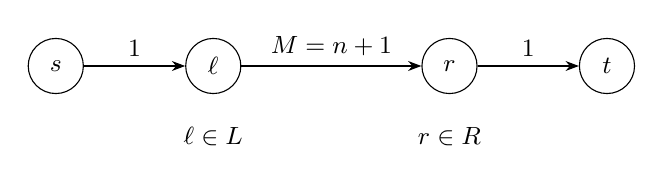
\begin{tikzpicture}[>=Stealth,vertex/.style={circle,draw,minimum size=7mm},
 every node/.style={font=\small}]
 \node[vertex] (s) at (0,0) {$s$};
 \node[vertex] (l) at (2,0) {$\ell$};
 \node[vertex] (r) at (5,0) {$r$};
 \node[vertex] (t) at (7,0) {$t$};
 \draw[->] (s) -- node[above] {$1$} (l);
 \draw[->] (l) -- node[above] {$M=n+1$} (r);
 \draw[->] (r) -- node[above] {$1$} (t);
 \node[below=3mm of l] {$\ell\in L$};
 \node[below=3mm of r] {$r\in R$};
\end{tikzpicture}
\end{center}
Compute a maximum flow and a corresponding minimum cut
$(U,\overline U)$, with $s\in U$ and $t\notin U$.
Return
\[
 \boxed{C=(L\setminus U)\cup(R\cap U).}
\]
Thus a left vertex is selected on the sink side, and a right vertex
is selected on the source side.

\textbf{Why a minimum cut cannot cross a middle arc.}
The cut with source side $\{s\}$ has capacity $|L|\le n<M$.
Any cut crossing an arc $\ell\to r$ has capacity at least $M$.
Hence no minimum cut crosses such an arc. In particular,
\[
 \ell\in L\cap U,\quad \{\ell,r\}\in E
 \quad\Longrightarrow\quad r\in R\cap U.
\]

\textbf{The returned set is a cover of the same size as the cut.}
For each edge $\{\ell,r\}$, either $\ell\notin U$, so $\ell\in C$,
or $\ell\in U$, which forces $r\in U$ and hence $r\in C$.
Thus $C$ covers every edge. As no middle arc crosses the cut,
\[
 \capc(U,\overline U)
 =|L\setminus U|+|R\cap U|=|C|.
\]

\textbf{Every vertex cover yields a cut of the same capacity.}
For any cover $D\subseteq L\cup R$, define
\[
 U_D=\{s\}\cup(L\setminus D)\cup(R\cap D).
\]
A middle arc could cross this cut only if both its endpoints were
outside $D$, contradicting that $D$ covers every edge.
The crossing outer arcs are exactly $s\to\ell$ for $\ell\in L\cap D$
and $r\to t$ for $r\in R\cap D$. Therefore
$\capc(U_D,\overline{U_D})=|D|$.
By the minimality of $(U,\overline U)$, $|C|\le|D|$ for every cover
$D$. This proves that the reduction returns a \emph{minimum} vertex cover.

\textbf{Implementation and complexity.}
Obtain $U$ by residual reachability from $s$ after maximum flow.
The network has $n+2$ vertices and $m+n$ arcs; construction and
recovery cost $O(n+m)$ time and space.
An integer augmenting-path implementation makes at most
$\min\{|L|,|R|\}$ augmentations, because each adds at least one unit
and the total flow is at most this quantity. Including the final search,
the time is $O((n+m)(1+\min\{|L|,|R|\}))$, with $O(n+m)$ space.
The empty graph returns the empty cover directly.

\newpage
\exercise{7.30}{Hall's theorem}
Let $G=(L\cup R,E)$ be bipartite with $|L|=|R|=n$. For
$A\subseteq L$, define its neighborhood by
\[
 N(A)=\{r\in R:\text{some $\ell\in A$ satisfies $\{\ell,r\}\in E$}\}.
\]
We prove
\[
 \boxed{\text{$G$ has a perfect matching}
 \quad\Longleftrightarrow\quad
 |N(A)|\ge|A|\ \text{for every }A\subseteq L.}
\]
When $n=0$, both statements hold trivially, using the empty matching.

\textbf{Necessity.}
Suppose a perfect matching exists. For any $A\subseteq L$, the
matching assigns its $|A|$ vertices to $|A|$ distinct vertices in
$N(A)$. Hence $|N(A)|\ge|A|$.

\textbf{Sufficiency: construct a network.}
Assume the neighborhood condition holds. Add $s,t$ and the arcs
\[
 s\to\ell\ (\text{capacity }1),\qquad
 \ell\to r\ (\text{capacity }n+1)\ \text{for }\{\ell,r\}\in E,
 \qquad r\to t\ (\text{capacity }1).
\]
The cut with source side $\{s\}$ has capacity $n$.
We show that \emph{every} $s$--$t$ cut has capacity at least $n$.

Let $U$ be any source side of a cut, and put
$A=U\cap L$, $B=U\cap R$. There are two cases:
\begin{enumerate}[label=(\roman*)]
 \item If a middle arc $\ell\to r$ crosses from $U$ to
       $\overline U$, the cut capacity is at least $n+1>n$.
 \item Otherwise every neighbor of $A$ belongs to $B$, so
       $N(A)\subseteq B$. Only outer arcs cross, giving
       \[
        \capc(U,\overline U)
        =n-|A|+|B|
        \ge n-|A|+|N(A)|
        \ge n.
       \]
\end{enumerate}
Therefore the minimum cut capacity is exactly $n$. By the
max-flow min-cut theorem, the maximum flow value is $n$.

\textbf{From a maximum flow to a perfect matching.}
All capacities are integers, so there exists an \emph{integral}
maximum flow. Since the $n$ arcs leaving $s$ each have capacity one,
a value-$n$ flow saturates every one of them. Similarly, it saturates
every arc entering $t$.
At each $\ell\in L$, conservation gives a total outgoing flow of
one. Integrality and nonnegativity imply that exactly one middle arc
from $\ell$ carries one unit. At each $r\in R$, exactly one middle
arc carries one unit into $r$.
Select precisely these unit-flow middle arcs. They are original
graph edges, no two share an endpoint, and every vertex is incident
to one of them. They therefore form a perfect matching.

\textbf{A certificate when Hall's condition fails.}
If some $A\subseteq L$ has $|N(A)|<|A|$, the source side
$U=\{s\}\cup A\cup N(A)$ defines a cut of capacity
\[
 n-|A|+|N(A)|<n.
\]
This cut prevents a value-$n$ flow and therefore prevents a perfect
matching, explicitly connecting Hall's obstruction to a deficient cut.

\vfill
{\footnotesize\textit{Source of exercise statements:}
S. Dasgupta, C. H. Papadimitriou, and U. V. Vazirani,
\textit{Algorithms}, Chapter 7, pp. 226, 229, and 231.
The solutions and proofs above are written for this assignment.}
\end{document}
